\documentclass[]{article}
\usepackage[utf8]{inputenc}
\usepackage[english]{babel}
\usepackage{graphicx}
\usepackage{hyperref}
\usepackage{appendix}
\hypersetup{
	colorlinks=true,
	linkcolor=blue,
	filecolor=magenta,      
	urlcolor=cyan,
}
\usepackage{mathtools}
\usepackage{float}   %this package is for placing graphs and tables in where the TeX is
\graphicspath{{images/}{../images/}}

\usepackage{blindtext}

\usepackage{subfiles}
\usepackage{verbatim}
\providecommand{\EqDir}{Equations}
\providecommand{\RefDir}{References}

\usepackage{apacite}


\title{A Replication of Carroll(1997}
\author{Yusuf Suha Kulu, Jeongwon (John) Son, and Mingzuo Sun}
\date{}

\begin{document}
\linespread{2}
\maketitle

\begin{align}
	c_t = \kappa_t[m_t + h_t]\\
	h_t = \sum_{i=t+1}^{\infty}R^{i-t}y_{i} \approx \frac{y_t}{r - g}\\
	\kappa = {(1 - {[R^{-1}(\beta R)^{1/\rho}]})}
\end{align}
\begin{align}
c_t = \kappa_t[m_t + h_t]\\
h_t = \sum_{i=t+1}^{T}R^{i-t}y_{i} \\
\kappa_t = \frac{(1 - {[R^{-1}(\beta R)^{1/\rho}]})}{(1 - {[R^{-1}(\beta R)^{1/\rho}]}^{T-t+1})}
\end{align}
\begin{align}
	1= R\beta E_{t-1}[\{c_t[R[m_{t-1}-c_{t-1}]/Gn_t + v_t]Gn_t/c_{t-1}\}^{-\rho}]
\end{align}
\begin{table}[H]
	\scalebox{.7}{\begin{tabular}{lrrrrrrr}
\toprule
{} &  Growth rate of aggregate consumption &  Average growth rate of household permanent income &  Average growth rate of household consumption &  Aggregate personal saving rate &  Average MPC out of wealth &  Average net wealth &  Target net wealth \\
\midrule
Base Value         &                              0.020957 &                                           0.014807 &                                      0.014978 &                        0.006265 &                   0.315820 &            0.341770 &           0.313770 \\
g = .04            &                              0.040290 &                                           0.034225 &                                      0.034508 &                        0.009891 &                   0.414938 &            0.265945 &           0.246728 \\
depreciation = .10 &                              0.020821 &                                           0.014807 &                                      0.015143 &                        0.004310 &                   0.477366 &            0.230806 &           0.214614 \\
\bottomrule
\end{tabular}
}
	\label{table:1}
      \end{table}
\begin{figure}[H]
	\centering
	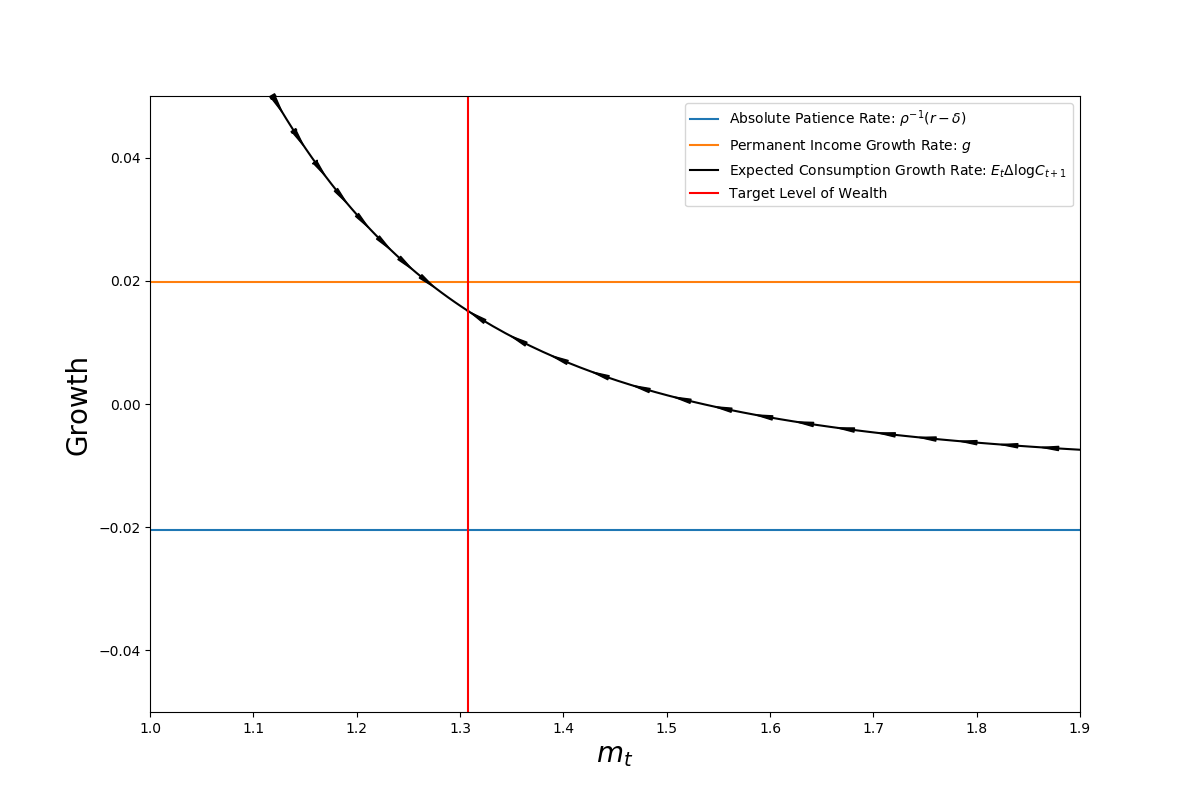
\includegraphics{Figures/Figure1a.png}
	\label{figure:1}
\end{figure}

\subfile{Appendix/Appendix}
%\bibliography{References/Aiyagari1994}

\end{document}